% =====================================================================
%  GNG/ELG 5301 -- Final Research Report (IEEE format, IEEEtran class)
%  AI-Powered Data Governance for PIPEDA Compliance in a Canadian Bank
%
%  DRAFT PREPARED WITH GENERATIVE-AI ASSISTANCE -- see the AI-use
%  statement (Appendix D). The team must review, rewrite the analysis in
%  its own words, verify every claim and citation, and complete the
%  author block before submission.
% =====================================================================
\documentclass[journal,onecolumn,11pt]{IEEEtran}

\usepackage[T1]{fontenc}
\usepackage{cite}
\usepackage{amsmath}
\usepackage{graphicx}
\usepackage{booktabs}
\usepackage{tabularx}
\usepackage{array}
\usepackage{multirow}
\usepackage{xcolor}
\usepackage{tikz}
\usetikzlibrary{positioning,arrows.meta,fit,backgrounds,calc}
\usepackage[hidelinks]{hyperref}
\usepackage{url}
\usepackage{longtable}

\newcolumntype{L}[1]{>{\raggedright\arraybackslash}p{#1}}
\newcolumntype{Y}{>{\raggedright\arraybackslash}X}
\renewcommand{\arraystretch}{1.15}
\setlength{\emergencystretch}{2em}

\begin{document}

\title{AI-Powered Data Governance for PIPEDA Compliance:\\
An Evidence-Based Assessment of OpenMetadata in a Canadian Bank}

\author{Kshitij~Vengurlekar, [Team Member~2], [Team Member~3], [Team Member~4], and~[Team Member~5]%
\thanks{GNG/ELG 5301 Professional Skills and Responsibility, University of Ottawa, Fall 2026. Instructor: Prof.\ M.\ Alnabhan.}%
\thanks{The organization studied, ``Borealis Bank of Canada,'' is fictional and all data are synthetic. Proof-of-concept code and evidence: \texttt{poc/} in the project repository.}}

\markboth{GNG/ELG 5301 Team Research Project --- Final Report}{Vengurlekar \MakeLowercase{\textit{et al.}}: AI-Powered Data Governance for PIPEDA Compliance}

\maketitle

% ---------------------------------------------------------------------
\begin{abstract}
\textbf{Problem.} Canadian banks hold large volumes of personal information in transactional (OLTP) systems and copy much of it into analytical (OLAP) warehouses, where it is reused for marketing, fraud and regulatory reporting. The \emph{Personal Information Protection and Electronic Documents Act} (PIPEDA) requires organizations to know where this information is, why it is held, who may use it and when it must be destroyed. Data-governance platforms now promise to automate much of this work with artificial intelligence (AI). \textbf{Question.} \emph{How, and with what professional safeguards, can a Canadian bank use an open-source, AI-assisted metadata platform to operationalize PIPEDA's fair information principles across its OLTP and OLAP data?} \textbf{Method.} We combined a structured review of 45 scholarly, regulatory, standards, professional and patent sources with a reproducible Docker proof of concept (POC) built on OpenMetadata~2.0.5 and a synthetic bank of 1,500 customers. Auto-classification was scored against column-level ground truth. \textbf{Findings.} Out-of-the-box AI classification found 72\% of personal-information columns and only 4 of 7 high-risk identifiers; several Canadian Social Insurance Numbers were caught only because Australian and U.S. patterns happened to match. Canada-specific recognizers raised recall to 100\% (F1 0.783$\rightarrow$0.943), and a human feedback workflow removed the remaining false positives. Metadata controls exposed planted PIPEDA defects (55 customers e-mailed after withdrawing consent, 38 records past retention, 1,239 stored card-verification values), but the platform governs the \emph{catalogue}, not the data: enforcement required tag-driven controls generated into the warehouse. \textbf{Implications and recommendations.} AI makes a personal-information inventory feasible at scale, but only as a supervised control: banks should (i) localize classifiers for Canadian identifiers, (ii) keep humans accountable for every classification decision, (iii) connect catalogue metadata to enforcement and testing, and (iv) govern AI assistants that query the catalogue as privileged users.
\end{abstract}

\begin{IEEEkeywords}
Data governance, PIPEDA, privacy, metadata management, data catalogs, auto-classification, personally identifiable information, OpenMetadata, Model Context Protocol, banking, professional responsibility.
\end{IEEEkeywords}

% =====================================================================
\section{Introduction and Problem Context}
\IEEEPARstart{A}{} Canadian bank's customer data rarely stays where it was collected. A Social Insurance Number (SIN) captured at account opening sits in a core-banking database, flows nightly into a dimensional warehouse \cite{kimball}, and from there into marts for marketing, anti-money-laundering (AML) reporting and analytics. Each copy is ``personal information'' under PIPEDA \cite{pipeda}, and each must respect the ten fair information principles of Schedule~1: accountability, identifying purposes, consent, limiting collection, limiting use and retention, accuracy, safeguards, openness, individual access, and challenging compliance. The professional problem is that most banks cannot answer basic questions about these copies: which columns hold personal information, why, who may read them, and when they should be deleted.

\subsection{Why it matters}
The consequences of not knowing are concrete. The Office of the Privacy Commissioner of Canada (OPC) found that the 2019 Desjardins breach, which exposed SINs, birth dates and transaction histories of about 9.7 million people, followed from failures of accountability, retention and safeguards, including data that were kept longer than necessary in two data warehouses that an insider could reach \cite{opc_desjardins}. Prudential regulators now expect the same discipline: OSFI Guideline B-13 requires federally regulated financial institutions to identify, classify and protect data by confidentiality and to run periodic discovery scans \cite{osfi_b13}, and Guideline E-23 (effective May 2027) extends model-risk management to AI systems \cite{osfi_e23}. Federal privacy reform is also in motion: Bill C-27 died in January 2025 and Bill C-36, the \emph{Protecting Privacy and Consumer Data Act}, received first reading in June 2026 \cite{billc36}. Meanwhile, privacy teams increasingly own AI governance \cite{iapp_ai}.

\subsection{Stakeholders}
The problem affects \emph{customers} (whose information is at risk), the \emph{Chief Privacy Officer} (CPO) who is accountable under Principle~4.1, \emph{data stewards and engineers} who build and document pipelines, \emph{business users} in marketing and AML who need data, \emph{regulators} (OPC, OSFI, FINTRAC), and \emph{executives} who carry legal, reputational and financial risk. Their interests partly conflict: business users want broad access, privacy staff want minimization, and engineers want automation that does not slow delivery.

\subsection{Objectives}
The project aims to (1) synthesize credible evidence on how AI-assisted metadata platforms support privacy compliance; (2) test those claims on a realistic but synthetic Canadian bank; (3) identify the professional responsibilities that AI features create rather than remove; and (4) recommend actionable steps for a bank's privacy and data leadership.

% =====================================================================
\section{Research Question and Scope}
\textbf{Primary question.} \emph{How, and with what professional safeguards, can a Canadian bank use an open-source, AI-assisted metadata platform (OpenMetadata) to operationalize PIPEDA's fair information principles across its OLTP and OLAP data?}

\textbf{Sub-questions.} SQ1: How accurately do AI auto-classification features locate personal information in Canadian banking data, and what improves them? SQ2: Which PIPEDA principles can catalogue metadata, workflows and tests support, and which remain outside their reach? SQ3: What accountability mechanisms must surround the AI features for the resulting controls to be professionally defensible?

\textbf{In scope.} Structured data in relational OLTP and OLAP stores; OpenMetadata 2.0.5 (open source) and its AI features (Presidio/spaCy-based auto-classification \cite{presidio}, recognizer-feedback workflows, the Model Context Protocol (MCP) server \cite{om_mcp}); PIPEDA and the federal financial-sector guidance that intersects it.

\textbf{Out of scope.} Unstructured documents and images; commercial catalogues (compared only through the literature); provincial private-sector laws such as Quebec's Law~25; legal advice. We do not collect human-participant data: the bank and all records are synthetic, in line with the course's research-ethics rules.

\textbf{Assumptions.} The bank's retention schedule (seven years after the end of a relationship) is an internal policy assumption consistent with FINTRAC's minimum five-year record-keeping rule \cite{fintrac_records}; Bill C-36 is treated as forthcoming, not as law.

% =====================================================================
\section{Method and Evidence Process}
\subsection{Search strategy and source selection}
We searched Crossref, Google Scholar, IEEE Xplore, the ACM Digital Library, SpringerLink, arXiv, Google Patents, the Justice Laws website, and the websites of the OPC, OSFI, FINTRAC, NIST, ISO, BIS and IAPP between October 15 and 21, 2026. Search strings combined three concept blocks: (\emph{data governance} OR \emph{data catalog} OR \emph{metadata} OR \emph{lineage}) AND (\emph{privacy} OR \emph{PIPEDA} OR \emph{personal information} OR \emph{PII}) AND (\emph{automat*} OR \emph{machine learning} OR \emph{AI} OR \emph{classification}). The search log is in Appendix~B.

Inclusion criteria were: peer-reviewed or authoritative (regulator, standards body, recognized professional association, granted patent, or official product documentation); directly relevant to a sub-question; and verifiable through a DOI, publisher record or official URL. We excluded vendor marketing, undated web content, and any reference we could not verify. Every DOI was checked against Crossref metadata and every URL was retrieved on October~21, 2026. Forty-five sources were retained: 11 journal articles, 2 conference papers and preprints, 4 handbooks and technical books, 10 statutes, bills and regulator publications, 8 standards and technical reports, 3 patents, 1 professional publication, and 6 technical documentation sources (Appendix~A).

\subsection{Evidence organization and analytical approach}
Each source was coded in an evidence table (source, type, focus, key finding, relevance, limitation, theme) using six themes: T1 governance structures and accountability; T2 automated discovery and classification; T3 metadata, lineage and catalogues as compliance infrastructure; T4 Canadian regulatory expectations; T5 human oversight of automation; T6 enforcement and the policy-to-data gap. The synthesis (Section~IV) is organized by these themes, not by source.

\subsection{Proof of concept as a structured test}
Because the literature contains few column-level evaluations of PII classifiers on structured banking data (see Section~IV-B), we built a small, reproducible POC to test specific claims. It is not a production system. Its design follows the course's advice that technical artifacts should serve the research question.

\emph{Environment.} The official OpenMetadata 2.0.5 Docker Compose stack (server, PostgreSQL metadata store, Elasticsearch) plus a PostgreSQL~16 instance hosting the fictional bank: an OLTP database (\texttt{core\_banking}, 10 tables) and a Kimball-style OLAP warehouse (\texttt{bank\_dw}, 9 tables). Everything runs on a laptop in a 4\,GB Docker VM with one command (\texttt{scripts/run\_poc.sh}).

\emph{Data.} A seeded generator created 1,500 customers, 2,336 accounts, 1,239 cards, 7,500 consent records, 55,058 transactions, 516 support tickets and 400 rows of a ``legacy credit-union import'' whose columns were never renamed (\texttt{fld\_01}--\texttt{fld\_04}). No real person is represented (reserved \texttt{example.*} e-mail domains, the fictional 555-01XX telephone exchange, random Luhn-valid identifiers). We deliberately planted defects that a PIPEDA program should detect: an ETL bug that keeps customers in a marketing audience after they withdraw consent; customers closed more than seven years ago; stored card-verification values (CVVs); and malformed postal codes.

\emph{Ground truth and metrics.} Every one of the 145 columns was labelled \textbf{H} (high-risk identifier: SIN, card number, CVV, account or government-ID number; 7 columns), \textbf{D} (direct identifier: name, e-mail, phone, address, postal code, birth date, IP address, free text containing these; 18), \textbf{Q} (quasi-identifier; 10), \textbf{F} (financial; 5) or \textbf{N} (not personal; 105). A column flagged as sensitive was scored as a true positive if its label was H or D. We report precision, recall and F1 for three configurations: the out-of-the-box \texttt{PII} classification, a Canada-tuned \texttt{PIPEDA} classification, and the tuned classification after one round of human feedback.

% =====================================================================
\section{Evidence Synthesis}
\subsection{T1 --- Data governance is a system of decision rights, not a tool}
The literature agrees that data governance assigns decision rights and accountability for data assets \cite{khatri,abraham,otto}. Khatri and Brown frame it as decisions about data principles, quality, metadata, access and life cycle \cite{khatri}; Abraham et al.'s review of 145 publications adds that governance mechanisms must be structural (roles), procedural (policies, processes) and relational (communication) \cite{abraham}. Practitioner bodies of knowledge make the same point \cite{dmbok}, and ISO/IEC 38505-1 places accountability for data with the governing body \cite{iso38505}. PIPEDA encodes this directly: Principle~4.1 requires a designated accountable individual. The consistent implication is that a catalogue can \emph{record} decision rights (owners, stewards, reviewers) but cannot \emph{create} them. Janssen et al.\ argue that trustworthy AI depends on this foundation, because algorithmic systems inherit the quality and provenance of their data \cite{janssen}.

\subsection{T2 --- Automated discovery works, but is context-dependent}
Automated discovery of sensitive data is an active area of practice and invention: patents cover context-aware neural detection \cite{pat_ibm} and confidence scoring of personal-information findings \cite{pat_bigid}, and Capital One reports that character-level neural models can classify sensitive columns at production throughput \cite{truong}. Yet three limitations recur. First, models trained on one jurisdiction's identifiers do not transfer: Truong et al.\ stress the scarcity of labelled financial datasets \cite{truong}. Second, sensitivity is contextual: the OPC treats financial information as generally sensitive but insists the assessment depends on circumstances \cite{opc_sensitive}. Third, combinations of individually harmless fields re-identify people: Sweeney's \emph{k}-anonymity work and Rocher et al.'s generative model show that a handful of quasi-identifiers (birth date, postal code, sex) identify most individuals \cite{sweeney,rocher}. A classifier that labels columns one at a time cannot see this combination risk. We found no peer-reviewed benchmark of column-level PII classification on Canadian banking schemas; this evidence gap motivated the POC.

\subsection{T3 --- Metadata, lineage and catalogues are compliance infrastructure}
Data catalogues improve findability and reuse of enterprise data \cite{labadie}. Provenance research distinguishes \emph{why}, \emph{where} and \emph{how} lineage \cite{herschel}; for privacy, ``where'' lineage is what lets a bank answer an individual-access request (Principle~4.9) or scope a breach. BCBS~239 requires banks to aggregate risk data with documented lineage and controls \cite{bcbs239}, but a 2023 progress report found most global systemically important banks still had substantial work to do \cite{bcbs_progress}, which suggests that lineage at scale remains hard. Data contracts \cite{jones_contracts} and data-mesh ``federated computational governance'' \cite{dehghani} propose expressing obligations as machine-checkable rules. Because data quality is multi-dimensional and judged by fitness for use \cite{wangstrong}, such rules must encode the purpose of the data, not only its format. The common thread is \emph{policy as metadata}: obligations become effective only when they are attached to specific assets and tested.

\subsection{T4 --- Canadian expectations converge on inventory, purpose and safeguards}
PIPEDA's principles \cite{pipeda}, the OPC's consent guidelines (express consent for sensitive information or unexpected uses) \cite{opc_consent}, breach record-keeping for 24 months \cite{breachregs}, OSFI B-13's classification and discovery-scan expectations \cite{osfi_b13}, and FINTRAC's five-year record and large-cash-reporting rules \cite{fintrac_records,fintrac_lctr} all presuppose an accurate inventory of personal information tied to purposes and retention periods. International frameworks agree: the NIST Privacy Framework's ``Identify-P'' function \cite{nist_pf} and Privacy by Design's ``privacy as the default'' \cite{cavoukian}. There is \emph{tension} as well as convergence: FINTRAC requires retention that PIPEDA's limiting-retention principle would otherwise minimize, so retention rules must be purpose-specific rather than global.

\subsection{T5 --- Human oversight is necessary but fragile}
AI-governance literature locates AI governance inside corporate, IT and data governance \cite{mantymaki} and frameworks require human accountability for AI outputs \cite{nist_airmf,iso42001,osfi_e23}. Human-factors research warns that oversight degrades into \emph{automation bias}: people over-trust reliable automation and stop checking it \cite{parasuraman}. The IAPP reports that privacy and legal functions now hold primary responsibility for AI governance in many organizations \cite{iapp_ai}, which places privacy professionals in the loop of AI classification decisions. The disagreement in the literature is about degree: vendors and patents emphasize automated confidence thresholds \cite{pat_bigid}, whereas regulators and standards emphasize documented human review \cite{osfi_e23,nist_airmf}.

\subsection{T6 --- The policy-to-data gap and new AI interfaces}
Attribute-based access control (ABAC) lets policies key off attributes such as classification tags \cite{nist800162}, and patents describe deriving access policies from tags and lineage \cite{pat_hitachi}. But a catalogue's policies typically govern the catalogue itself; the OpenMetadata documentation is explicit that contract ``security'' sections are documentation, not enforcement \cite{om_contracts}. A newer risk arises from AI assistants: MCP lets large-language-model agents call catalogue tools \cite{om_mcp}, and a systematic study identifies tool poisoning, over-privileged servers and data exfiltration among its threats \cite{hou_mcp}.

\subsection{Patterns across themes}
Table~\ref{tab:synthesis} condenses the synthesis. Three patterns stand out. First, every source family converges on the need for an \emph{inventory} of personal information tied to accountable owners, but they disagree on how much of that inventory can be produced automatically: patents and industry research are optimistic, regulators are cautious, and academic work warns about context and combination effects. Second, findings are strongly \emph{context-dependent}: classifier performance, sensitivity, and even retention obligations change with jurisdiction and purpose. Third, a recurring and under-studied risk is the distance between \emph{described} controls (metadata, contracts, policies in a catalogue) and \emph{enforced} controls (permissions and transformations in the data platform itself).

\begin{table}[!t]
\caption{Synthesis: Where the Evidence Converges, Diverges and Is Missing}
\label{tab:synthesis}
\centering\small
\begin{tabularx}{\linewidth}{L{2.7cm} Y Y Y}
\toprule
\textbf{Theme} & \textbf{Convergence} & \textbf{Divergence or tension} & \textbf{Implication for a Canadian bank} \\
\midrule
T1 Accountability & Governance assigns decision rights; a named person is accountable \cite{khatri,abraham,pipeda,iso38505} & Centralized vs.\ federated (domain) models \cite{otto,dehghani} & Catalogue records ownership; it cannot create it \\
T2 Automated discovery & Automation is necessary at bank scale \cite{truong,pat_ibm,pat_bigid} & Optimistic vendor claims vs.\ contextual sensitivity and re-identification \cite{opc_sensitive,sweeney,rocher} & Measure classifiers locally; treat combinations separately \\
T3 Metadata as infrastructure & Lineage and catalogues enable access requests, reporting and audits \cite{labadie,herschel,bcbs239} & Lineage is hard to complete in practice \cite{bcbs_progress} & Register every pipeline that moves PI \\
T4 Canadian expectations & Inventory, purpose, retention and safeguards \cite{opc_consent,osfi_b13,nist_pf} & PIPEDA minimization vs.\ FINTRAC retention \cite{fintrac_records} & Purpose-specific retention rules \\
T5 Human oversight & Humans remain accountable for AI outputs \cite{nist_airmf,iso42001,osfi_e23} & Automated thresholds vs.\ documented review \cite{pat_bigid}; automation bias \cite{parasuraman} & Targeted, measured review of AI tags \\
T6 Enforcement gap & Attribute/tag-based control is feasible \cite{nist800162,pat_hitachi} & Catalogue policy $\neq$ data policy \cite{om_contracts}; new AI attack surface \cite{hou_mcp} & Generate enforcement from metadata; govern AI agents \\
\bottomrule
\end{tabularx}
\end{table}

\subsection{Evidence gaps}
We found (i) no published evaluation of OpenMetadata's classifier, (ii) no Canadian-identifier benchmark for structured data, and (iii) little empirical work on how privacy officers review AI-generated tags. We also found no independent, openly published evaluation of commercial governance platforms; analyst reports exist but are proprietary, so we did not rely on them. These gaps limit how far any conclusion can be generalized.

% =====================================================================
\section{Proof of Concept: Design and Results}
\begin{figure}[!t]
\centering
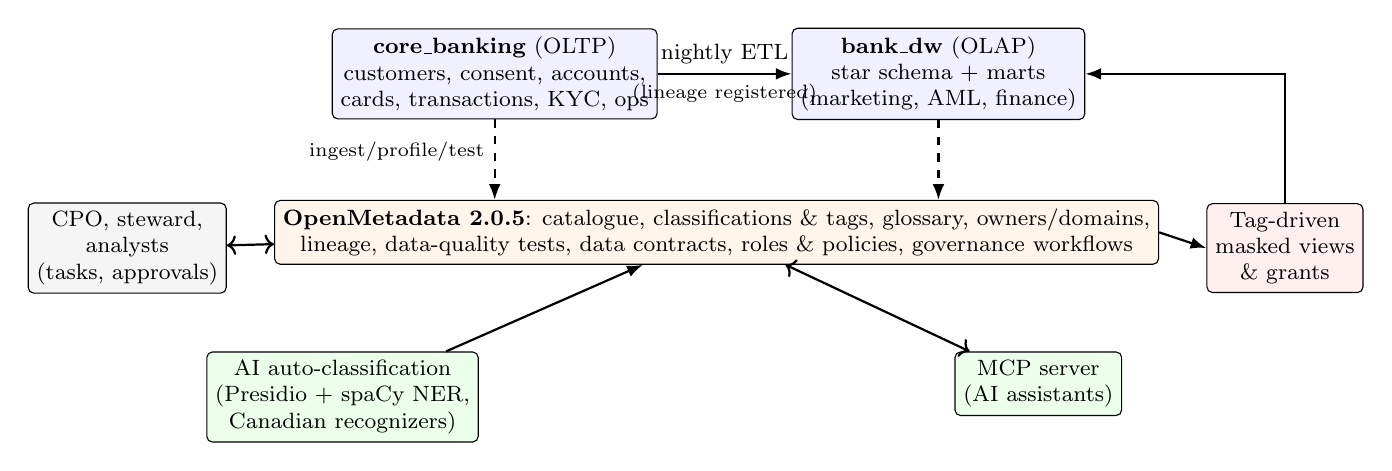
\begin{tikzpicture}[
  font=\footnotesize,
  box/.style={draw, rounded corners=2pt, align=center, minimum height=8mm, inner sep=3pt, fill=white},
  db/.style={box, fill=blue!6},
  om/.style={box, fill=orange!8},
  ai/.style={box, fill=green!8},
  person/.style={box, fill=gray!8},
  arr/.style={-{Latex[length=2mm]}, thick},
  darr/.style={-{Latex[length=2mm]}, thick, dashed}
]
\node[db] (oltp) {\textbf{core\_banking} (OLTP)\\customers, consent, accounts,\\cards, transactions, KYC, ops};
\node[db, right=1.7cm of oltp] (olap) {\textbf{bank\_dw} (OLAP)\\star schema + marts\\(marketing, AML, finance)};
\draw[arr] (oltp) -- node[above]{nightly ETL} node[below]{\scriptsize (lineage registered)} (olap);
\node[om, below=1.6cm of $(oltp)!0.5!(olap)$, minimum width=8.6cm] (om) {\textbf{OpenMetadata 2.0.5}: catalogue, classifications \& tags, glossary, owners/domains,\\lineage, data-quality tests, data contracts, roles \& policies, governance workflows};
\node[ai, below left=1.1cm and -2.6cm of om] (cls) {AI auto-classification\\(Presidio + spaCy NER,\\Canadian recognizers)};
\node[ai, below right=1.1cm and -2.6cm of om] (mcp) {MCP server\\(AI assistants)};
\node[person, left=0.6cm of om, yshift=-0.2cm] (people) {CPO, steward,\\analysts\\(tasks, approvals)};
\node[box, fill=red!6, right=0.6cm of om, yshift=-0.2cm] (enf) {Tag-driven\\masked views\\\& grants};
\draw[darr] (oltp.south) -- node[left, pos=0.4]{\scriptsize ingest/profile/test} (om.north -| oltp.south);
\draw[darr] (olap.south) -- (om.north -| olap.south);
\draw[arr] (cls) -- (om);
\draw[arr, <->] (mcp) -- (om);
\draw[arr, <->] (people) -- (om);
\draw[arr] (om.east) -- (enf.west);
\draw[arr] (enf.north) |- (olap.east);
\end{tikzpicture}
\caption{POC architecture. OpenMetadata reads both databases with a read-only principal; AI classification proposes tags; people approve or correct them through workflows; tags then drive tests, policies, and generated database controls.}
\label{fig:arch}
\end{figure}

Fig.~\ref{fig:arch} summarizes the architecture. The governance model mapped each PIPEDA principle to concrete platform objects (Table~\ref{tab:mapping}). All entities were created through the OpenMetadata REST API so the configuration is version-controlled and repeatable.

\begin{table}[!t]
\caption{Mapping PIPEDA Schedule 1 Principles to POC Controls}
\label{tab:mapping}
\centering\small
\begin{tabularx}{\linewidth}{L{3.4cm} Y}
\toprule
\textbf{Principle} & \textbf{OpenMetadata control implemented in the POC} \\
\midrule
4.1 Accountability & Privacy Office team; CPO owns the \texttt{PIPEDA} classification and glossary; every table has an owning team and domain. \\
4.2 Identifying purposes & \texttt{PIPEDAPurpose} tags (account servicing, fraud prevention, regulatory reporting, marketing, analytics) on all 14 governed tables; purpose stated in a data contract. \\
4.3 Consent & Consent replicated to the warehouse; data-quality tests on the marketing mart; consent row filter in generated views. \\
4.4 Limiting collection & AI classification inventory of high-risk identifiers; test that no CVVs are stored. \\
4.5 Limiting use and retention & Table \texttt{retentionPeriod} (e.g., P7Y, P90D); tests for records past retention. \\
4.6 Accuracy & Format and uniqueness tests (postal code, e-mail, SIN). \\
4.7 Safeguards & Five-level sensitivity tags (HighRisk, DirectIdentifier, QuasiIdentifier, Financial, NonPersonal); tag-conditioned deny rules; tag-integrity rule; generated masked views. \\
4.8 Openness & 13-term PIPEDA glossary approved through the glossary approval workflow. \\
4.9 Individual access & Column-level lineage from OLTP to every mart through a registered ETL pipeline; MCP lineage queries. \\
4.10 Challenging compliance & Recognizer-feedback workflow (steward reports, CPO decides) with a task audit trail. \\
\bottomrule
\end{tabularx}
\end{table}

\subsection{Result 1: Out-of-the-box classification is not Canadian-aware}
OpenMetadata's auto-classification scans column names and sampled values with Microsoft Presidio recognizers and a spaCy named-entity model \cite{om_autoclass,presidio}. Its 40 predefined recognizers in version 2.0.5 target U.S., U.K., Australian, Indian, Spanish, Italian and other identifiers; none targets the Canadian SIN, Canadian postal codes, provincial driver's licences or Canadian passports. On our data the baseline achieved precision 0.857 and recall 0.720 (Table~\ref{tab:cls}). The detail is more revealing than the totals: the SIN column was tagged only because an \emph{Australian Tax File Number} pattern happened to match the NNN-NNN-NNN format, the unlabelled legacy SIN column was caught by a \emph{U.S. ABA routing-number} pattern, and telephone numbers were flagged by a \emph{U.K. NHS-number} recognizer. Dates of birth were tagged \emph{non-sensitive} by a generic date recognizer, while postal codes, account numbers and passport or licence numbers were missed. Correct outcomes for the wrong reasons are fragile: a format change would silently break them.

\begin{table}[!t]
\caption{AI Auto-Classification Against Ground Truth (145 Columns; Positive = H or D)}
\label{tab:cls}
\centering\small
\begin{tabular}{lcccccc}
\toprule
\textbf{Configuration} & \textbf{Precision} & \textbf{Recall} & \textbf{F1} & \textbf{FP} & \textbf{FN} & \textbf{High-risk found} \\
\midrule
Out-of-the-box \texttt{PII} & 0.857 & 0.720 & 0.783 & 3 & 7 & 4 of 7 \\
Canada-tuned \texttt{PIPEDA} & 0.893 & 1.000 & 0.943 & 3 & 0 & 7 of 7 \\
Tuned + one round of steward feedback & 1.000 & 1.000 & 1.000 & 0 & 0 & 7 of 7 \\
\bottomrule
\end{tabular}
\end{table}

\begin{figure}[!t]
\centering
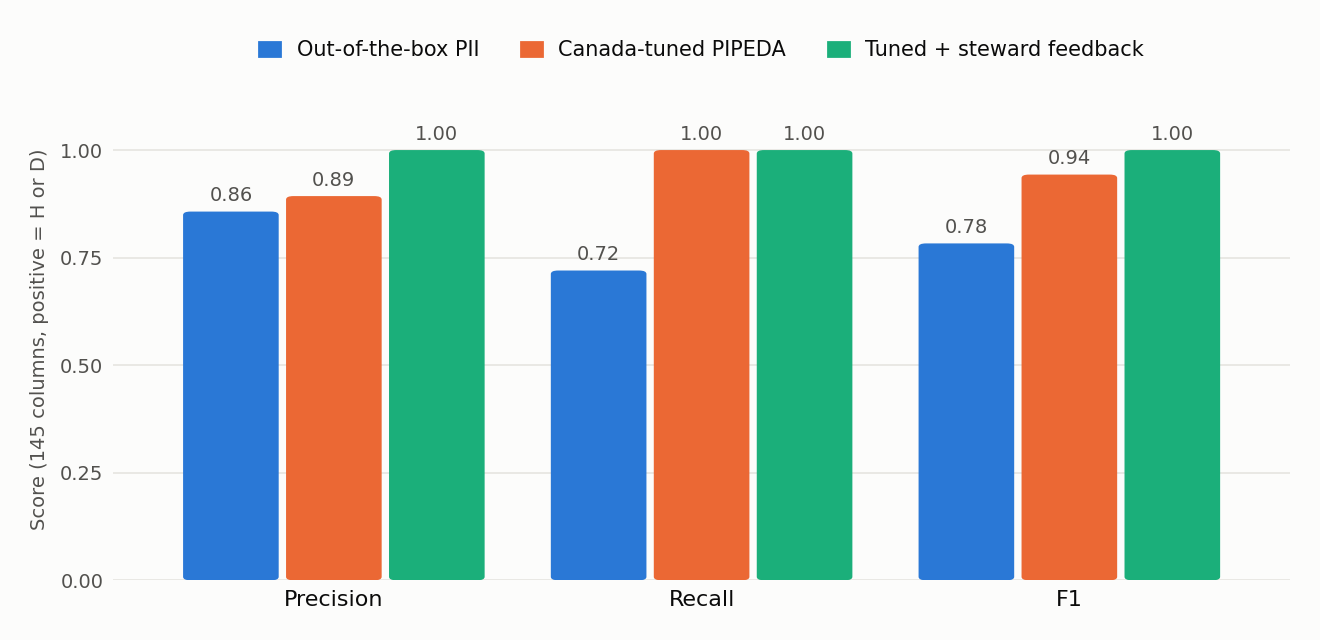
\includegraphics[width=0.78\linewidth]{figures/classification_comparison.png}
\caption{Precision, recall and F1 of the three classification configurations (same data, same ground truth).}
\label{fig:cls}
\end{figure}

\subsection{Result 2: Localization works, but required working around the product}
We created a mutually exclusive \texttt{PIPEDA} classification whose tags carry 17 recognizers: regular expressions for formatted and unformatted SINs (with column-name context), Canadian postal codes, Ontario licences and Canadian passports; column-name rules; and selected Presidio recognizers. Recall rose to 1.000 and F1 to 0.943 (Table~\ref{tab:cls}, Fig.~\ref{fig:cls}); all seven high-risk columns were found, including the SINs hidden in \texttt{fld\_02}. Two product limitations surfaced. First, the open-source \texttt{metadata classify} command hard-codes the built-in \texttt{PII} classification \cite{om_source}, so recognizers on any other classification are silently ignored; we reused the official workflow class with a different classification filter (about 20 lines of code). Second, ``custom'' recognizers with validation code are not implemented, so SINs cannot be checksum-validated and any nine-digit pattern may match. These are exactly the kind of undocumented gaps a professional must test for before relying on a tool.

\subsection{Result 3: Human feedback corrects errors and leaves a record}
The tuned classifier's three false positives were \texttt{city} columns that the spaCy model read as person names. A data steward reported each as a false positive through the recognizer-feedback API, which started OpenMetadata's built-in \texttt{RecognizerFeedbackReviewWorkflow}; the CPO approved each task; the platform removed the tags and added a column-level exception to the responsible recognizer. A re-run produced no false positives against the H/D threshold (Table~\ref{tab:cls}). Exact five-level class accuracy, however, rose only from 0.959 to 0.966: once the person-name recognizer was excepted, a broader column-name rule re-tagged all three \texttt{city} columns as quasi-identifiers, which is correct for customer city but not for branch cities, which are public business addresses. Correcting one error exposed the over-breadth of another rule; feedback is an iterative process, not a one-time fix. Every AI-generated tag remains in the \emph{Suggested} state until a person confirms it, which is the appropriate default for an accountable process. The glossary approval workflow behaved similarly: 13 PIPEDA terms were created in review and the CPO approved them; we also observed that editing a term under review cancels its approval task, a sensible safeguard that prevents approval of content that has changed.

\subsection{Result 4: A living inventory of personal information}
Combining the confirmed classifications with ownership, domain, purpose, retention and lineage metadata produced the inventory in Table~\ref{tab:inventory} and the flow map in Fig.~\ref{fig:flow}, both generated from the OpenMetadata API rather than maintained by hand. Two observations matter for PIPEDA. First, the inventory immediately exposed over-collection: the legacy import table holds SINs under meaningless column names and has no identified purpose, so its retention was set to zero (\texttt{P0D}) pending deletion, and the card table stores CVVs that should never be retained. Second, the flow map shows that direct identifiers (names, e-mail addresses, dates of birth) propagate from the OLTP customer table into three warehouse objects, whereas the SIN does not leave the OLTP layer. That is the kind of evidence a bank needs to answer an individual-access request (Principle~4.9) or to scope a breach notification under the real-risk-of-significant-harm test \cite{breachregs}.

\begin{table}[!t]
\caption{Personal-Information Inventory Generated from the Catalogue}
\label{tab:inventory}
\centering\footnotesize
\begin{tabularx}{\linewidth}{L{6.1cm} L{2.3cm} Y c L{2.2cm}}
\toprule
\textbf{Table} & \textbf{Sensitivity (roll-up)} & \textbf{Purposes} & \textbf{Retention} & \textbf{Owner} \\
\midrule
\texttt{core.customer} & HighRisk & Account servicing & P7Y & Data Engineering \\
\texttt{core.customer\_consent} & --- & Account servicing & P7Y & Privacy Office \\
\texttt{core.account} & HighRisk & Account servicing & P7Y & Data Engineering \\
\texttt{core.card} & HighRisk & Account servicing & P2Y & Data Engineering \\
\texttt{core.transaction} & DirectIdentifier & Account servicing, fraud prevention & P7Y & Data Engineering \\
\texttt{kyc.identity\_document} & HighRisk & Regulatory reporting & P5Y & Fraud \& AML \\
\texttt{ops.support\_ticket} & DirectIdentifier & Account servicing & P2Y & Data Engineering \\
\texttt{ops.legacy\_member\_import} & HighRisk & \emph{none identified} & P0D & Data Engineering \\
\texttt{dw.dim\_customer} & DirectIdentifier & Analytics & P7Y & Data Engineering \\
\texttt{dw.dim\_consent} & --- & Marketing, analytics & P7Y & Privacy Office \\
\texttt{dw.fact\_transaction} & Financial & Analytics, fraud prevention & P7Y & Data Engineering \\
\texttt{mart.marketing\_campaign\_audience} & DirectIdentifier & Marketing & P90D & Retail Marketing \\
\texttt{mart.aml\_large\_cash\_txn} & DirectIdentifier & Regulatory reporting & P5Y & Fraud \& AML \\
\texttt{mart.monthly\_branch\_activity} & Financial & Analytics & P10Y & Data Engineering \\
\bottomrule
\end{tabularx}
\end{table}

\begin{figure}[!t]
\centering
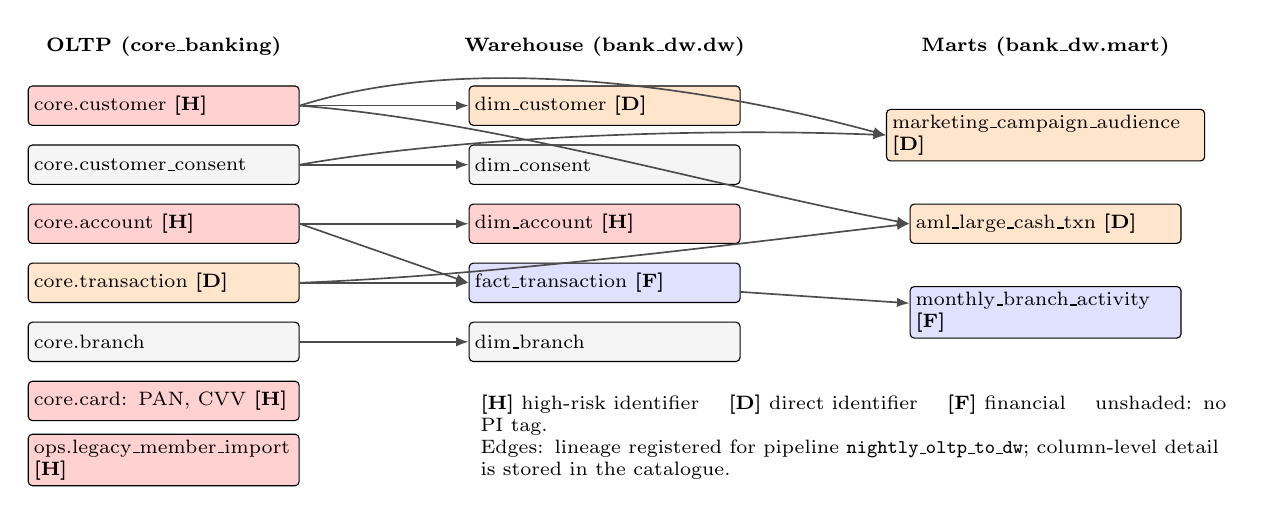
\begin{tikzpicture}[
  font=\scriptsize,
  t/.style={draw, rounded corners=1.5pt, text width=3.3cm, minimum height=5mm, inner sep=2pt, align=left},
  H/.style={t, fill=red!18}, D/.style={t, fill=orange!20}, F/.style={t, fill=blue!12}, N/.style={t, fill=gray!8},
  e/.style={-{Latex[length=1.6mm]}, semithick, gray!60!black}
]
% column x positions (node centres)
\def\xa{0}\def\xb{5.6}\def\xc{11.2}
\node[font=\scriptsize\bfseries] at (\xa,0.75) {OLTP (core\_banking)};
\node[font=\scriptsize\bfseries] at (\xb,0.75) {Warehouse (bank\_dw.dw)};
\node[font=\scriptsize\bfseries] at (\xc,0.75) {Marts (bank\_dw.mart)};
\node[H] (cust) at (\xa,0)     {core.customer \textbf{[H]}};
\node[N] (cons) at (\xa,-0.75) {core.customer\_consent};
\node[H] (acct) at (\xa,-1.5)  {core.account \textbf{[H]}};
\node[D] (txn)  at (\xa,-2.25) {core.transaction \textbf{[D]}};
\node[N] (br)   at (\xa,-3.0)  {core.branch};
\node[H] (card) at (\xa,-3.75) {core.card: PAN, CVV \textbf{[H]}};
\node[H] (leg)  at (\xa,-4.5)  {ops.legacy\_member\_import \textbf{[H]}};
\node[D] (dc)   at (\xb,0)     {dim\_customer \textbf{[D]}};
\node[N] (dcon) at (\xb,-0.75) {dim\_consent};
\node[H] (da)   at (\xb,-1.5)  {dim\_account \textbf{[H]}};
\node[F] (ft)   at (\xb,-2.25) {fact\_transaction \textbf{[F]}};
\node[N] (db)   at (\xb,-3.0)  {dim\_branch};
\node[D, text width=3.9cm] (mk)   at (\xc,-0.375){marketing\_campaign\_audience \textbf{[D]}};
\node[D] (aml)  at (\xc,-1.5)  {aml\_large\_cash\_txn \textbf{[D]}};
\node[F] (mb)   at (\xc,-2.625){monthly\_branch\_activity \textbf{[F]}};
\draw[e] (cust) -- (dc);  \draw[e] (cons) -- (dcon); \draw[e] (acct) -- (da);
\draw[e] (txn) -- (ft);   \draw[e] (acct.east) -- (ft.west); \draw[e] (br) -- (db);
\draw[e] (cust.east) .. controls +(2.2,0.7) and +(-2.2,0.6) .. (mk.west);
\draw[e] (cons.east) .. controls +(2.0,0.35) and +(-2.4,0.1) .. (mk.west);
\draw[e] (cust.east) .. controls +(2.5,-0.2) and +(-2.6,0.5) .. (aml.west);
\draw[e] (txn.east)  .. controls +(2.5,0.1) and +(-2.6,-0.3) .. (aml.west);
\draw[e] (ft) -- (mb);
\node[align=left, anchor=north west, text width=9.5cm] at (\xb-1.7,-3.55) {%
\textbf{[H]} high-risk identifier \quad \textbf{[D]} direct identifier \quad \textbf{[F]} financial \quad unshaded: no PI tag.\\
Edges: lineage registered for pipeline \texttt{nightly\_oltp\_to\_dw}; column-level detail is stored in the catalogue.};
\end{tikzpicture}
\caption{Personal-information flow map derived from catalogue lineage and the most sensitive column tag of each table. The card and legacy tables have no downstream copies; the SIN stays in the OLTP layer.}
\label{fig:flow}
\end{figure}

\subsection{Result 5: Metadata tests exposed planted PIPEDA defects}
Twelve data-quality tests, each named after the principle it checks, ran through OpenMetadata's test framework (Table~\ref{tab:dq}); failures automatically opened six incidents in the Incident Manager. The most instructive result concerns consent: a naive test that the audience's \texttt{consent\_marketing} flag is true \emph{passed}, while a test that cross-checks the audience against current consent state \emph{failed} with 55 customers who had withdrawn consent. Compliance testing therefore needs the business rule, not just the column. The e-mail format test also failed for 240 addresses containing accented characters from French names: a case where a ``failure'' may reflect an over-strict rule rather than bad data, and where human judgement must decide.

\begin{table}[!t]
\caption{PIPEDA Data-Quality Tests in the POC}
\label{tab:dq}
\centering\small
\begin{tabularx}{\linewidth}{L{2.6cm} L{4.3cm} c Y}
\toprule
\textbf{Principle} & \textbf{Test (table)} & \textbf{Status} & \textbf{Observed} \\
\midrule
4.3 Consent & Audience flag \texttt{consent\_marketing} is true (mart) & Pass & 611 of 611 rows \\
4.3 Consent & Audience cross-checked against consent state (mart) & \textbf{Fail} & 55 customers withdrew consent but remain \\
4.3 Consent & Withdrawal after capture; purpose not null (OLTP) & Pass & 0 violations \\
4.4 Limiting collection & No CVV stored (\texttt{core.card}) & \textbf{Fail} & 1,239 rows \\
4.4 Minimization & Warehouse keeps only 3-character FSA & Pass & --- \\
4.5 Retention & Closed customers past 7 years purged (OLTP and DW) & \textbf{Fail} & 38 rows in each \\
4.6 Accuracy & Canadian postal-code format (OLTP) & \textbf{Fail} & 17 of 1,500 invalid \\
4.6 Accuracy & E-mail format (OLTP) & \textbf{Fail} & 240 non-ASCII; rule under review \\
4.6 Accuracy & SIN uniqueness (OLTP) & Pass & 1,473 unique \\
FINTRAC & Large-cash mart contains only $\geq$\,\$10,000 & Pass & 0 violations \\
\bottomrule
\end{tabularx}
\end{table}

\subsection{Result 6: Catalogue policies work only on the catalogue}
Tag-conditioned OpenMetadata policies behaved as designed once correctly attached: a marketing analyst was denied (HTTP~403) sample data, queries and profiles of tables tagged \texttt{PIPEDA.HighRisk} or \texttt{PIPEDA.DirectIdentifier}, while AML and privacy staff were allowed; and an organization-wide rule prevented anyone outside the Privacy and Data Governance offices from changing PIPEDA tags. Two findings temper this. First, the sample-data endpoint evaluated \texttt{matchAnyTag()} only against \emph{table-level} tags, whereas the built-in permission debugger also counted column tags and reported ``denied'' when the endpoint allowed access; we therefore rolled the most sensitive column tag up to each table. Second, and more fundamentally, none of these policies stops a SQL user from querying the warehouse \cite{om_contracts}. We closed the loop with a script that reads tags and purposes from the OpenMetadata API and generates PostgreSQL views and grants per business role: high-risk columns are dropped, direct identifiers are pseudonymized unless the table's purpose matches the role's purpose, and marketing views apply a current-consent row filter. The marketing role then saw 556 audience rows instead of 611, exactly removing the 55 withdrawn customers, and was denied access to the raw schemas.

\subsection{Result 7: AI assistants can answer privacy questions --- and change metadata}
OpenMetadata's built-in MCP server exposed 15 tools. Through it, an AI assistant answered privacy-office questions grounded in the catalogue: which tables hold high-risk identifiers, where a customer's e-mail address flows (lineage through the registered ETL pipeline), whether the marketing mart passes its consent tests, and what ``real risk of significant harm'' means in the bank's glossary. The same server also exposes write tools (\texttt{patch\_entity}, \texttt{create\_entity}, \texttt{create\_lineage}), so an agent connected with an over-privileged token could alter the very tags that drive safeguards, a concrete instance of the MCP threats catalogued by Hou et al.\ \cite{hou_mcp}.

% =====================================================================
\section{Analysis}
\subsection{Answering the research question}
Combining the literature with the POC, our answer is that an AI-assisted metadata platform can operationalize PIPEDA's principles \emph{as a supervised control system}, not as an autonomous one. It is strongest where principles reduce to knowing and documenting: inventory (4.4), purpose (4.2), openness (4.8) and lineage for access requests and breach scoping (4.9). It is useful but incomplete for consent, retention and accuracy (4.3, 4.5, 4.6), where it can \emph{detect} violations but the fix lies in pipelines and business processes. It is weakest for safeguards (4.7) unless catalogue metadata is wired into enforcement points the platform does not control.

\subsection{SQ1: Accuracy is a property of the deployment, not the product}
The jump from F1 0.783 to 0.943 came from local knowledge (Canadian formats and naming) rather than from more sophisticated AI. This supports the literature's view that classifier performance is context-dependent \cite{truong,opc_sensitive} and implies that vendor accuracy claims are not transferable evidence. It also reframes the professional question: a bank that deploys a classifier without measuring it on its own schemas cannot know its false-negative rate, and false negatives, unlike false positives, are invisible. Our measured gains are optimistic (the same people wrote the generator and the recognizers), but the direction is robust: none of the baseline's Canadian-identifier hits relied on a Canadian rule.

\subsection{SQ2: Metadata detects, people and pipelines correct}
The consent result illustrates the central analytic point. The defect was visible only because consent state had been replicated, lineage documented and a cross-table rule written; a column-level check would have certified a non-compliant mart. Metadata platforms therefore shift effort from \emph{finding} problems to \emph{specifying} obligations precisely, which echoes the ``policy as metadata'' theme \cite{jones_contracts,dehghani}. They also make obligations auditable: each failed test opened an incident with an owner. What they cannot do is decide whether 240 accented e-mail addresses are an accuracy problem or an over-strict rule; that judgement belongs to accountable people.

\subsection{SQ3: Human oversight must be designed, not assumed}
OpenMetadata's defaults (tags as suggestions, reviewer-gated glossaries, feedback workflows with audit trails) embody good oversight design. But the literature on automation bias warns that a reviewer who approves hundreds of correct suggestions will eventually stop checking \cite{parasuraman}. Oversight must therefore be targeted (review high-risk and low-confidence tags first), measured (track reviewer override rates), and periodically challenged with planted test cases, much as our ground truth did.

\subsection{Alternative interpretations}
One could argue that the POC shows the tool ``works'' and the remaining issues are configuration details. We disagree on two grounds. The undocumented hard-coded classification filter and the table-versus-column policy discrepancy are behaviours a reasonable administrator would not anticipate; relying on them without testing would be negligent. And the most consequential defects (consent, retention, CVV storage) were found by tests that encode legal reasoning, not by AI. A second interpretation is that commercial platforms avoid these limitations; we found no independent, openly published evidence for that claim, and the professional obligation to verify would be the same.

% =====================================================================
\section{Professional Responsibility Implications}
\textbf{Accountability.} Delegating classification to AI does not delegate accountability: PIPEDA Principle~4.1 and OSFI E-23 both require a named human owner of outcomes \cite{pipeda,osfi_e23}. The CPO must own the classification taxonomy and the recognizer configuration as controlled artefacts, with change approval.

\textbf{Privacy and data minimization.} Auto-classification samples real rows and can store them in the catalogue. Sample storage should be disabled or masked for high-risk tables, or the catalogue becomes another copy of the data it is meant to protect, the same pattern that magnified the Desjardins breach \cite{opc_desjardins}.

\textbf{Security.} Metadata is security-relevant: whoever can remove a tag can disable a safeguard. Tag-integrity rules, separation of duties, alerting on tag changes, and least-privilege tokens for ingestion bots and AI agents are required \cite{osfi_b13,hou_mcp}.

\textbf{Fairness and equity.} Recognizer quality varies by name origin and language; spaCy mis-read city names as people, and accented French names failed a naive e-mail rule. Controls that work less well for some customers (for example francophone or immigrant customers) create unequal privacy protection and should be tested for.

\textbf{Professional obligations and honesty.} Engineers and privacy professionals must report limitations they discover, including to the open-source maintainers, rather than presenting a tool as compliant. Equally, results from synthetic data must be presented as such.

\textbf{Organizational and public impact.} A bank that can trace personal information end-to-end can honour access requests, scope breaches quickly and demonstrate compliance to regulators. Over-reliance on automation, in contrast, risks a false sense of compliance that is worse than acknowledged ignorance.

% =====================================================================
\section{Recommendations}
Recommendations are addressed to the CPO (accountable executive), the Chief Data Officer (CDO) and data-platform engineering, and are sequenced by horizon. Each is traceable to a finding (Table~\ref{tab:roadmap}); Table~\ref{tab:raci} proposes who is responsible (R), accountable (A), consulted (C) and informed (I) for the recurring governance activities, including the AI components.

\begin{table}[!t]
\caption{Recommendation Roadmap Traced to Evidence}
\label{tab:roadmap}
\centering\small
\begin{tabularx}{\linewidth}{c L{4.1cm} L{1.8cm} L{1.7cm} Y}
\toprule
\textbf{\#} & \textbf{Action} & \textbf{Owner} & \textbf{Horizon} & \textbf{Evidence (finding / source)} \\
\midrule
1 & Measure classifier on labelled local schemas & CDO & 0--3 mo & Result 1; \cite{truong,opc_sensitive} \\
2 & Add Canadian recognizers; verify they run & Data platform & 0--3 mo & Results 1--2; \cite{om_source} \\
3 & Human confirmation of high-risk tags & CPO & 0--3 mo & Result 3; \cite{parasuraman,osfi_e23} \\
4 & Lock down metadata and AI-agent access & Security & 0--3 mo & Results 6--7; \cite{hou_mcp,osfi_b13} \\
5 & PIPEDA rules as tests and contracts & Data stewards & 3--12 mo & Result 5; \cite{jones_contracts,opc_consent} \\
6 & Generate enforcement from metadata & Data platform & 3--12 mo & Result 6; \cite{nist800162,om_contracts} \\
7 & Complete pipeline lineage & Data engineering & 3--12 mo & T3; \cite{herschel,bcbs_progress} \\
8 & Quasi-identifier combination reviews & Privacy office & 3--12 mo & T2; \cite{sweeney,rocher} \\
9 & Classifier under model-risk management & Model risk & 12+ mo & T5; \cite{osfi_e23,nist_airmf} \\
10 & Bill C-36 readiness using catalogue evidence & CPO & 12+ mo & T4; \cite{billc36} \\
11 & Upstream fixes and Canadian recognizers & Engineering & 12+ mo & Results 2, 6 \\
\bottomrule
\end{tabularx}
\end{table}

\begin{table}[!t]
\caption{Proposed RACI for AI-Assisted Privacy Governance}
\label{tab:raci}
\centering\footnotesize
\begin{tabular}{lccccc}
\toprule
\textbf{Activity} & \textbf{CPO} & \textbf{Steward} & \textbf{Engineer} & \textbf{Business user} & \textbf{AI component} \\
\midrule
Maintain classification taxonomy and recognizers & A & R & C & I & --- \\
Propose sensitivity tags & I & C & I & --- & R (suggests only) \\
Confirm or reject high-risk tags & A & R & I & --- & --- \\
Report a misclassification & I & R & R & R & --- \\
Approve glossary terms and purposes & A/R & C & I & C & --- \\
Register lineage and retention for pipelines & I & C & A/R & --- & --- \\
Investigate failed PIPEDA tests (incidents) & A & R & R & I & --- \\
Grant data access (generated controls) & A & C & R & I & --- \\
Answer catalogue questions via MCP & I & C & --- & R & R (read-only) \\
\bottomrule
\end{tabular}
\end{table}

\subsection{Immediate (0--3 months)}
\begin{enumerate}
\item \textbf{Measure before you trust (CDO).} Build a labelled sample of real schemas, as our ground truth did, and report precision and recall of auto-classification, with recall on high-risk identifiers as the acceptance criterion.
\item \textbf{Localize the classifier (data platform).} Add Canadian recognizers (SIN, postal code, provincial health and licence numbers, passport, transit/institution/account formats) and column-name rules for legacy naming; verify that the deployed version actually evaluates them.
\item \textbf{Keep AI tags as suggestions (CPO).} Require human confirmation for high-risk tags; use the feedback workflow for corrections so that every decision is attributable.
\item \textbf{Lock down metadata (security).} Apply tag-integrity rules, roll sensitivity up to table level for policy evaluation, disable sample storage for high-risk tables, and connect AI assistants only through least-privilege, read-only identities.
\end{enumerate}

\subsection{Medium term (3--12 months)}
\begin{enumerate}\setcounter{enumi}{4}
\item \textbf{Codify PIPEDA as tests (data stewards).} Express consent, retention and minimization rules as data-quality tests and data contracts on every mart that holds personal information, with incident ownership.
\item \textbf{Close the policy-to-data gap (data platform).} Generate warehouse masking, row filters and grants from catalogue tags and purposes, and alert when catalogue and database permissions diverge.
\item \textbf{Complete lineage (data engineering).} Register every pipeline that moves personal information so that access requests and breach scoping can be answered from lineage.
\item \textbf{Assess combination risk (privacy office).} Review tables that combine several quasi-identifiers, which column-level classifiers cannot judge \cite{sweeney,rocher}.
\end{enumerate}

\subsection{Longer term (12+ months)}
\begin{enumerate}\setcounter{enumi}{8}
\item \textbf{Treat the classifier as a model (model-risk management).} Bring it under OSFI E-23 governance: inventory, validation, monitoring and periodic re-testing.
\item \textbf{Prepare for Bill C-36 (CPO).} Use the catalogue's purpose and lineage records as the evidence base for whatever accountability and de-identification obligations the successor law imposes \cite{billc36}.
\item \textbf{Contribute upstream (engineering).} Report the hard-coded classification filter and policy-evaluation discrepancy to the OpenMetadata project, and contribute Canadian recognizers, reducing risk for the whole sector.
\end{enumerate}

% =====================================================================
\section{Limitations}
\textbf{Synthetic data and optimistic scores.} The bank, its schemas and its defects were designed by the authors, who also wrote the recognizers; the tuned and post-feedback scores are therefore upper bounds, and real legacy systems will be messier. \textbf{Small sample.} With 145 columns and 25 positives, a single misclassification moves recall by four points; no confidence intervals are claimed. \textbf{Single product and version.} Findings describe OpenMetadata 2.0.5 open source in its default configuration; later releases or commercial editions may differ. \textbf{Structured data only.} Documents, images and free-text archives, where much sensitive information lives, were out of scope. \textbf{Scripted personas.} Approvals were scripted to make the POC reproducible; they demonstrate workflow mechanics, not real reviewer behaviour. \textbf{Legal interpretation.} Mappings to PIPEDA reflect the authors' reading of public guidance, not legal advice; the law may change with Bill C-36. \textbf{Evidence base.} Few peer-reviewed studies evaluate catalogue-based privacy controls, and commercial-platform evidence is largely proprietary.

% =====================================================================
\section{Conclusion}
AI-assisted metadata platforms can give a Canadian bank something PIPEDA has always required but few banks have achieved: a living inventory of personal information linked to purposes, owners, lineage, tests and retention rules. Our evidence shows that this capability is real but conditional. Out of the box, the AI did not recognize Canadian identifiers; with local tuning and human feedback it did, and metadata tests exposed consent, retention and collection failures that a column-level view would miss. The platform, however, governs descriptions of data rather than the data itself, and its newest interface, AI assistants through MCP, is also a new attack surface. The defensible course is to treat AI classification as a monitored model inside an accountable governance system: measure it, localize it, keep people responsible for its decisions, and connect its outputs to real enforcement.

% =====================================================================
\section*{Acknowledgment}
The authors thank the GNG/ELG 5301 teaching team for feedback. See Appendix~D for the generative-AI use statement.

\bibliographystyle{IEEEtran}
\bibliography{references}

% =====================================================================
\appendices
\section{Evidence Table (Abbreviated)}
\label{app:evidence}
{\footnotesize
\begin{longtable}{L{2.3cm} L{1.7cm} L{4.4cm} L{4.6cm} L{0.8cm}}
\toprule
\textbf{Source} & \textbf{Type} & \textbf{Key finding} & \textbf{Relevance / limitation} & \textbf{Theme} \\
\midrule
\endhead
Khatri \& Brown \cite{khatri} & Journal & Five decision domains incl.\ metadata, access, life cycle & Foundational; pre-dates AI catalogues & T1 \\
Abraham et al.\ \cite{abraham} & Journal & Structural, procedural, relational mechanisms (145 sources) & Strong review; not finance-specific & T1 \\
Otto \cite{otto} & Journal & Organizational forms of data governance & Single-industry case & T1 \\
Janssen et al.\ \cite{janssen} & Journal & 13 principles for governing data for trustworthy AI & Public-sector focus & T1, T5 \\
DAMA \cite{dmbok} & Handbook & Data-management body of knowledge & Practitioner consensus & T1, T3 \\
Truong et al.\ \cite{truong} & Preprint & Neural column classification at bank scale & Industry, not peer-reviewed & T2 \\
IBM patent \cite{pat_ibm} & Patent & Context-aware BiLSTM detection with retraining & Claims, not evaluation & T2 \\
BigID patent \cite{pat_bigid} & Patent & Confidence levels for PI findings & Commercial claims & T2, T5 \\
Sweeney \cite{sweeney}; Rocher et al.\ \cite{rocher} & Journal & Quasi-identifiers re-identify individuals & Motivates combination risk & T2 \\
OPC bulletin \cite{opc_sensitive} & Regulator & Sensitivity is contextual; financial data generally sensitive & Non-binding guidance & T2, T4 \\
Labadie et al.\ \cite{labadie} & Conference & Catalogue initiatives and enterprise value & Little privacy evidence & T3 \\
Herschel et al.\ \cite{herschel} & Journal & Taxonomy of provenance & Technical survey & T3 \\
BCBS 239 \cite{bcbs239,bcbs_progress} & Standard / report & Lineage and aggregation duties; slow adoption & Bank-specific & T3, T4 \\
Jones \cite{jones_contracts}; Dehghani \cite{dehghani} & Books & Contracts and computational governance & Practitioner, limited evaluation & T3, T6 \\
PIPEDA \cite{pipeda}; regs \cite{breachregs} & Statute & Ten principles; 24-month breach records & Binding law & T4 \\
OPC Desjardins \cite{opc_desjardins} & Regulator & Breach from accountability, retention, safeguard gaps & Canadian bank precedent & T4, T6 \\
OSFI B-13 \cite{osfi_b13}; E-23 \cite{osfi_e23} & Regulator & Classification, discovery scans; AI model risk & FRFI scope & T4, T5 \\
FINTRAC \cite{fintrac_records,fintrac_lctr} & Regulator & 5-year records; \$10k LCTR & Conflicts with minimization & T4 \\
Bill C-36 \cite{billc36} & Bill & Proposed successor to PIPEDA Part 1 & Not law & T4 \\
NIST PF \cite{nist_pf}; PbD \cite{cavoukian} & Standards & Inventory, privacy by default & Voluntary & T4 \\
Mäntymäki et al.\ \cite{mantymaki} & Journal & AI governance within data/IT governance & Conceptual & T5 \\
Parasuraman \& Riley \cite{parasuraman} & Journal & Automation bias and misuse & Not privacy-specific & T5 \\
NIST AI RMF \cite{nist_airmf}; ISO 42001 \cite{iso42001} & Standards & Human oversight of AI & Voluntary & T5 \\
IAPP \cite{iapp_ai} & Professional & Privacy/legal lead AI governance (22\% each) & Survey, self-report & T5 \\
NIST ABAC \cite{nist800162}; Hitachi patent \cite{pat_hitachi} & Standard / patent & Attribute- and lineage-driven access control & Design, not evaluation & T6 \\
Hou et al.\ \cite{hou_mcp} & Journal & MCP threat taxonomy & Fast-moving field & T6 \\
OpenMetadata docs \cite{om_autoclass,om_policies,om_contracts,om_mcp}; source \cite{om_source} & Documentation & Product behaviour (verified in POC) & Vendor-maintained & T2, T6 \\
\bottomrule
\end{longtable}
}

\section{Search Log (Summary)}
\label{app:search}
{\footnotesize
\begin{tabularx}{\linewidth}{L{2.6cm} Y L{1.3cm} L{1.0cm}}
\toprule
\textbf{Database / site} & \textbf{Query (abridged)} & \textbf{Screened} & \textbf{Kept} \\
\midrule
Crossref, Scholar & ``data governance'' AND (framework OR review) & 40 & 5 \\
Crossref, IEEE, ACM & (``data catalog'' OR lineage OR provenance) AND (enterprise OR privacy) & 30 & 3 \\
Scholar, arXiv & (PII OR ``sensitive data'') AND (detection OR classification) AND (column OR structured OR financial) & 35 & 3 \\
Crossref, IEEE & ``automation bias''; AI AND privacy AND compliance checking & 15 & 1 \\
arXiv, ACM & ``Model Context Protocol'' AND security & 12 & 1 \\
Google Patents & sensitive data detection; personal information confidence; tag lineage access control & 25 & 3 \\
Justice Laws, OPC, OSFI, FINTRAC, Parliament & PIPEDA; consent; sensitive; Desjardins; B-13; E-23; record keeping; C-36 & 22 & 10 \\
NIST, ISO, BIS, IPC & privacy framework; AI RMF; 27701; 42001; 38505; BCBS 239; Privacy by Design & 18 & 8 \\
IAPP, Gartner, publishers & AI governance report; governance platforms; data contracts; data mesh; DMBOK; Kimball & 15 & 5 \\
OpenMetadata, Microsoft & auto-classification; roles and policies; data contracts; MCP; Presidio & 10 & 6 \\
\bottomrule
\end{tabularx}
}

\section{Reproducibility}
\label{app:repro}
The POC runs end-to-end with \texttt{poc/scripts/run\_poc.sh} (about 15--20 minutes on a laptop with Docker Desktop and 4\,GB of VM memory). It uses the unmodified official OpenMetadata 2.0.5 compose file plus an overlay; all generated evidence (classification snapshots, workflow audit, access-control results, enforcement checks, MCP transcript, compliance summary) is written to \texttt{poc/results/}. A full reset-and-rerun reproduced every figure reported here.

\section{Generative-AI Use Statement}
\label{app:ai}
\textbf{[To be completed and verified by the team before submission.]} Tool: Claude (Anthropic), used through Claude Code on October 21, 2026. Purpose: assistance with building the proof-of-concept code, locating candidate sources, and producing a first draft of this report. Verification: every reference was checked against a DOI, publisher record or official URL; every POC number was regenerated by a clean re-run; the team must (i) re-read each cited source to confirm it supports the claim attached to it, (ii) rewrite the analysis, professional-responsibility and recommendation sections in its own words and judgement, and (iii) record individual contributions. AI did not replace source evaluation, interpretation or authorship responsibilities, which remain with the team.

\end{document}
